%%%%%%%%%%%%%%%%%%%%%%%%%%%%%%%%%%%%%%%%%%%%%%%%%%%%%%%%%%%%%%%%%%%%%%%%%%%%%%%
%     STYLE POUR LES EXPOSÉS TECHNIQUES
%         3e année INSA de Rennes
%
%             NE PAS MODIFIER
%%%%%%%%%%%%%%%%%%%%%%%%%%%%%%%%%%%%%%%%%%%%%%%%%%%%%%%%%%%%%%%%%%%%%%%%%%%%%%%

\documentclass[a4paper,11pt]{article}

\usepackage{exptech}       % Fichier (./exptech.sty) contenant les styles pour
                           % l'expose technique (ne pas le modifier)


%\linespread{1,6}          % Pour une version destinée à un relecteur,
                           % décommenter cette commande (double interligne)

% UTILISEZ SPELL (correcteur orthographique) à accès simplifié depuis XEmacs


%\setlength{\parskip}{2ex}
\usepackage{color}
\usepackage{graphicx}
\definecolor{simColor}{rgb}{0.0, 0.5, 0.0}
\definecolor{dissimColor}{rgb}{0.8, 0.0, 0.0}
\definecolor{otherSimColor}{rgb}{0.0, 0.28, 0.67}

%%%%%%%%%%%%%%%%%%%%%%%%%%%%%%%%%%%%%%%%%%%%%%%%%%%%%%%%%%%%%%%%%%%%%%%%%%%%%%%

\title{ \textbf{Data Carving applied to small memory dumps} }
\markright{\'Etude pratique - Data carving}
                           % Pour avoir le titre de l'expose sur chaque page

\author{Alexandre \textsc{Audinot}, Thierry \textsc{Gaugry}, \\
        Nicolas \textsc{Hurman}, Gabriel \textsc{Prevosto} \\
        \\
        Encadrant : Gildas \textsc{Avoine}}

\date{}                    % Ne pas modifier

%%%%%%%%%%%%%%%%%%%%%%%%%%%%%%%%%%%%%%%%%%%%%%%%%%%%%%%%%%%%%%%%%%%%%%%%%%%%%%%

\begin{document}

\maketitle                 % Génère le titre
\thispagestyle{empty}      % Supprime le numéro de page sur la 1re page



\begin{abstract}
Nous possédons une multitude d'appareils que nous utilisons chaque jour, parfois à notre insu. Quelles informations enregistrent-ils ?
Au cours de cette étude pratique, nous avons essayé de développer un logiciel permettant de comprendre la structure d'une mémoire de petite taille, comme on peut en trouver dans des cartes de transport, des pass de ski ou encore dans l'électronique embarquée de nos véhicules. En appliquant une série d'algorithmes et à travers une interface intuitive, disséquer ce type de support devient une tâche plus simple et accessible.
\end{abstract}

\section{Introduction}
  \subsection{Contexte}
  \subsection{Etude de l'existant}
\section{Cahier des charges}
  \subsection{Spécifications originales}
  \subsection{État final}
\section{Présentation du logiciel}
  \subsection{Technologies utilisées}
  \subsection{Interface}
  \subsection{Fonctionnalités}
\section{Algorithmique}
  \subsection{Aide à la décision}
  \subsection{Analyse} Cet outil permet d'appliquer plusieurs algorithmes aux dumps, afin d'aider au repérage de l'information recherchée.

\subsubsection{Similarities \cite {ref-vandeursen}} \label{04-similarities}

Cet algorithme permet de mettre en évidence, dans un groupe de dumps, les chaînes de bits semblables (que nous appellerons similarités) ou dissemblables (que nous appellerons dissimilarités). Ces chaînes doivent être au même endroit dans chaque dump pour être reconnues.

Dans le cas de deux dumps, les similarités sont représentées par la couleur verte, tandis que les similarités sont représentées par la couleur rouge.

\begin{figure}[!h]
  \begin{center}
  {\tt\center
  {\color{simColor} Ce}{\color{dissimColor} ci es}{\color{simColor}t }{\color{dissimColor} un exemple de }{\color{simColor} similarité}

  {\color{simColor} Ce}{\color{dissimColor} la me}{\color{simColor}t }{\color{dissimColor} en couleur la }{\color{simColor} similarité}
  }
  \end{center}
  \caption{Exemple de similarités}
  \label{04-1-sim_simple}
\end{figure}

Afin d'affiner la recherche, il est possible de spécifier une taille de chaîne minimum :

\begin{figure}[!h]
  \begin{center}
  {\tt
  {\color{dissimColor} Ceci est un exemple de }{\color{simColor} similarité }{\color{dissimColor} avec une taille minimum de 4}

  {\color{dissimColor} Cela met en couleur la }{\color{simColor} similarité }{\color{dissimColor} faisant plus de 4 caractères}
  }
  \end{center}
  \caption{Similarités avec une taille de chaîne minimum}
  \label{04-1-sim_taille_min}
\end{figure}


Dans le cas de plusieurs dumps, on dispose de trois couleurs. Le rouge représente les dissimilarités, le vert les similarités concernant le dump visualisé (c'est-à dire les similarités commune à ce dump et à d'autres), tandis que le bleu correspond aux similarités ne concernant pas le dump visualisé (c'est-à dire les similarités communes à d'autres dumps).
Ces couleurs ont des nuances : plus le vert ou le bleu sont prononcés, plus il y a de dumps partageant la similarité en question.

\begin{figure}[!h]
  \begin{center}
  {\tt
  {\color{dissimColor} Encore un}{\color{otherSimColor} e au}{\color{dissimColor} tre }{\color{simColor} similarité}{\color{dissimColor} .}

  {\color{dissimColor} Toujours }{\color{simColor} plus }{\color{dissimColor} de }{\color{simColor} similarité}{\color{dissimColor} s}

  {\color{dissimColor} colorées }{\color{simColor} plus }{\color{dissimColor} qu'}{\color{otherSimColor} auparavant}{\color{dissimColor} .}
  }
  \end{center}
  \caption{Similatités entre trois dumps}
  \label{04-1-sim_mult}
\end{figure}

\subsubsection{Dotplot patterns \cite {ref-dotplot}} \label{04-dotplot}

Cet algorithme s'applique à deux dumps et génère un schéma similaire à celui ci-dessous :

\begin{figure}[!h]
  \begin{center}
  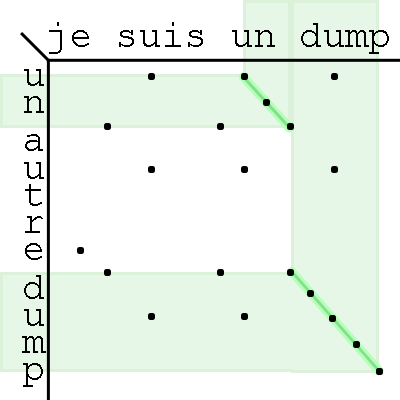
\includegraphics[scale=1]{res/04-2-dotplot.png}
  \caption{Un motif obtenu par dotplot}
  \label{04-1-dotplot}
  \end{center}
\end{figure}

Sur ce schéma, on retrouve l'un des dumps en abscisse, et l'autre en ordonnée. Les diagonales représentent des chaînes de bits semblables dans les deux dumps qui, contrairement aux similarités, ne sont pas nécessairement au même emplacement dans chaque dump. Leurs coordonnées représentent leurs positions dans chacun des dumps.

Dans cet exemple, on constate deux diagonales : l'une correspondant à la répétition du mot \texttt{un}, l'autre, plus longue, à celle du mot \texttt{dump}.

  \subsection{Pseudo-code}
  \subsection{Complexité}
  \subsection{Performances}
\section{Gestion du projet}
  \subsection{Outils}
  \subsection{Planification et réunions}
  \subsection{Versions intermédiaires}
  \subsection{Séparation du travail}
  \subsection{Distribution du temps}
\section{Conclusion}
  \subsection{Points remarquables au cours du projet}
  \subsection{Améliorations envisageables}
    1. Optimisations
    2. Masques préchargés
    3. Environnement plus intégré
    4. Davantage de visualisations
    5. Plugins pour les encodages
    6. Traduire le logiciel
\bibliography{biblio}

\end{document}
